\documentclass[tikz,border=6pt]{standalone}
\usepackage{amsmath,amssymb}
\usetikzlibrary{shapes.geometric,positioning,decorations.pathreplacing,calc}

\begin{document}
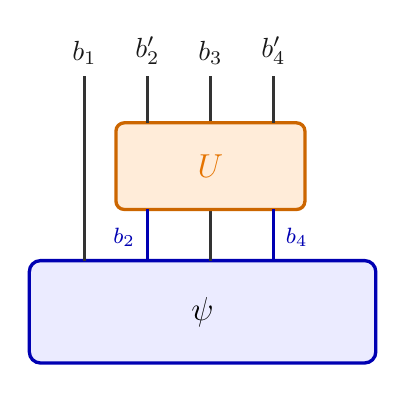
\begin{tikzpicture}[
    state/.style={draw=blue!70!black, fill=blue!8, rounded corners=4pt, line width=1.2pt, minimum height=1.3cm, align=center},
    gate/.style={draw=orange!80!black, fill=orange!15, rounded corners=3pt, line width=1.2pt, minimum height=1.1cm, align=center},
    leg/.style={line width=1.3pt, draw=black!80},
    contractleg/.style={line width=1.3pt, draw=blue!70!black},
    indexlabel/.style={font=\normalsize\color{black!90}}
]

    % State psi
    \node[state, minimum width=4.4cm] (psi) at (2.0, 0.8) {\large $\psi$};
    
    % Leg 1: bypasses U on the left
    \draw[leg] (0.5, 1.45) -- (0.5, 3.8) node[above, indexlabel] {$b_1$};
    
    % Leg 3: passes behind U (drawn first so U covers it)
    \draw[leg] (2.1, 1.45) -- (2.1, 3.8) node[above, indexlabel] {$b_3$};
    
    % Gate U (centered at x=2.1, spanning legs 2 and 4)
    \node[gate, minimum width=2.4cm] (U) at (2.1, 2.65) {\large\bfseries\color{orange!90!black} $U$};
    
    % Leg 2: enters U from psi
    \draw[contractleg] (1.3, 1.45) -- (1.3, 2.1);
    \node[font=\footnotesize\color{blue!70!black}, left=1pt] at (1.3, 1.75) {$b_2$};
    
    % Leg 4: enters U from psi
    \draw[contractleg] (2.9, 1.45) -- (2.9, 2.1);
    \node[font=\footnotesize\color{blue!70!black}, right=1pt] at (2.9, 1.75) {$b_4$};
    
    % Outgoing legs from U
    \draw[leg] (1.3, 3.2) -- (1.3, 3.8) node[above, indexlabel] {$b_2'$};
    \draw[leg] (2.9, 3.2) -- (2.9, 3.8) node[above, indexlabel] {$b_4'$};

\end{tikzpicture}
\end{document}
